 我々はまず、前立腺の病理画像をGP(Gleason pattern)に応じて正常腺管、GP3、GP4、GP5のセマンティックセグメンテーション(Semantic segmentation、画像を意味に基づいてピクセル単位で区分する手法)を行うU-Net\cite{unet}モデルを作成した。U-Netモデルは入力画像から次元を減らすエンコーダーと、減った次元を復元するデコーダーから構成される。エンコーダーにはVGG16\cite{vgg}を使用し、さらに転移学習を行っている。デコーダーの次元復元には逆畳込みではなくNearest samplingを用いた。\par

\vspace{0.5zh}

 モデルは当教室で診断された前立腺全摘出標本と、Fig\ref{fig:seg_color}のようなラベル付けによって訓練した。またモデルの出力例をFig\ref{fig:dl_sample}に示す。\par

\begin{figure}[htbp]\centering
  \begin{tabular}{c}
    \begin{subfigure}[t]{0.16\columnwidth}\centering
      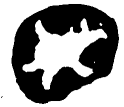
\includegraphics[width=0.7\columnwidth]{fig/gp_pin.png}
      \subcaption{正常腺管}
    \end{subfigure}

    \begin{subfigure}[t]{0.16\columnwidth}\centering
      
\includegraphics[width=0.7\columnwidth]{fig/gp_3_2.png}
      \subcaption{GP3:青}
    \end{subfigure}

    \begin{subfigure}[t]{0.16\columnwidth}\centering
      
\includegraphics[width=0.7\columnwidth]{fig/gp_4.png}
      \subcaption{GP4}
    \end{subfigure}

    \begin{subfigure}[t]{0.16\columnwidth}\centering
      
\includegraphics[width=0.7\columnwidth]{fig/gp_3_1.png}
      \subcaption{GP3+4}
    \end{subfigure}

    \begin{subfigure}[t]{0.16\columnwidth}\centering
      
\includegraphics[width=0.7\columnwidth]{fig/gp_5_2.png}
      \subcaption{GP5}
    \end{subfigure}

    \begin{subfigure}[t]{0.16\columnwidth}\centering
      
\includegraphics[width=0.7\columnwidth]{fig/gp_5_1.png}
      \subcaption{GP4+5}
    \end{subfigure}
  \end{tabular}
  \label{fig:example}
  \caption{セグメンテーションによる色分け例}
  \label{fig:seg_color}
\end{figure}

\begin{figure}[htbp]\centering
  \begin{tabular}{c}
    \begin{subfigure}[t]{0.33\columnwidth}\centering
      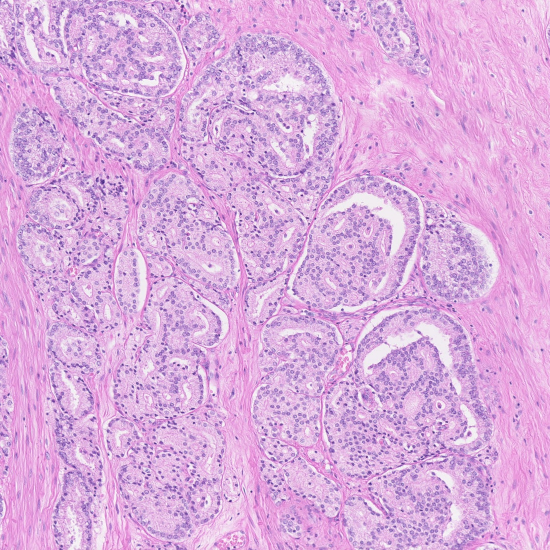
\includegraphics[width=0.9\columnwidth]{fig/fig_org.png}
      \subcaption{入力画像}
    \end{subfigure}

    \begin{subfigure}[t]{0.33\columnwidth}\centering
      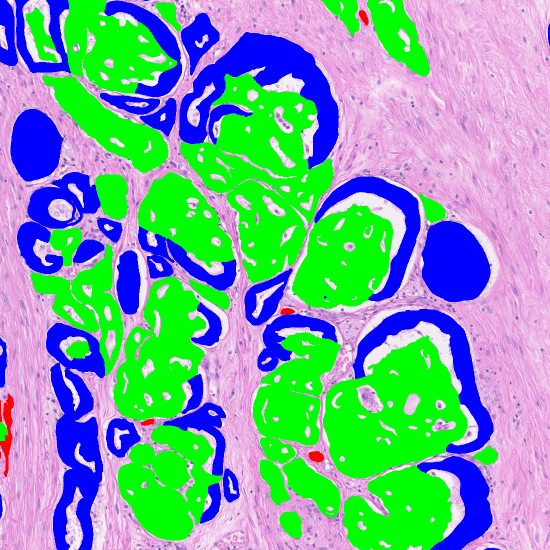
\includegraphics[width=0.9\columnwidth]{fig/fig_gt.png}
      \subcaption{ラベル画像}
    \end{subfigure}

    \begin{subfigure}[t]{0.33\columnwidth}\centering
      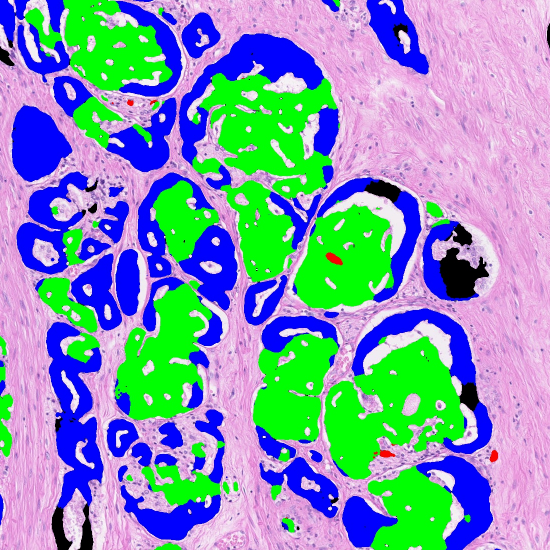
\includegraphics[width=0.9\columnwidth]{fig/fig_inf.png}
      \subcaption{出力画像}
    \end{subfigure}
  \end{tabular}
  \label{fig:example}
  \caption{U-Netモデルによる出力例}
  \label{fig:dl_sample}
\end{figure}

\vspace{0.5zh}

 さらに、USBカメラから入力された画像をネットワーク経由で送信するクライアントアプリケーションと、受信した画像をDLによって解析しその結果を配信するサーバーアプリケーションを作成した。前者は顕微鏡カメラとUSB接続したRaspberry Pi 4 Model Bに、後者はDLの動作するコンピュータにそれぞれ導入した。\par

\vspace{1zh}

\begin{figure}\centering
  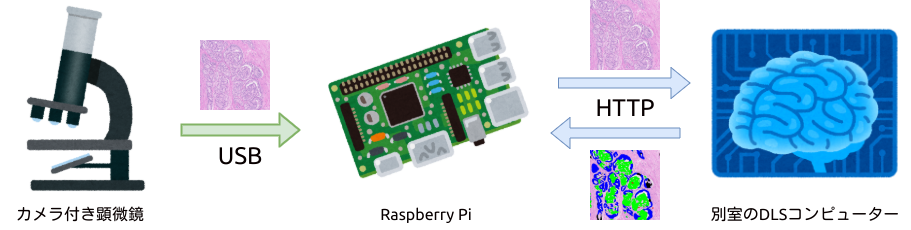
\includegraphics[width=\columnwidth]{fig/fig_arch.png}
  \caption{クライアント・サーバーアプリケーション構成図}
\end{figure}
\vspace{1zh}
